%%%%%%%%%%%%%%%%%%%%%%%%%%%%%%%%%%%%%%%%%%%%%%%%%%%%%%%%%%%%%%%%%%%%%%%%%%%%%%%%%%%%%%%%%%%%%%%%%%%%%%%%%%%%%%%%%%%%%%%%%%%%%%%%%%%%%%%%%%%%%%%%%%%%%%%%%%%%%%%%%%%
% Written By Michael Brodskiy
% Class: Circuits & Signals: Biomedical Applications
% Professor: N. Sun
%%%%%%%%%%%%%%%%%%%%%%%%%%%%%%%%%%%%%%%%%%%%%%%%%%%%%%%%%%%%%%%%%%%%%%%%%%%%%%%%%%%%%%%%%%%%%%%%%%%%%%%%%%%%%%%%%%%%%%%%%%%%%%%%%%%%%%%%%%%%%%%%%%%%%%%%%%%%%%%%%%%

\documentclass[12pt]{article} 
\usepackage{alphalph}
\usepackage[utf8]{inputenc}
\usepackage[russian,english]{babel}
\usepackage{titling}
\usepackage{amsmath}
\usepackage{graphicx}
\usepackage{enumitem}
\usepackage{amssymb}
\usepackage[super]{nth}
\usepackage{everysel}
\usepackage{ragged2e}
\usepackage{geometry}
\usepackage{multicol}
\usepackage{fancyhdr}
\usepackage{cancel}
\usepackage{siunitx}
\usepackage{physics}
\usepackage{tikz}
\usepackage{mathdots}
\usepackage{yhmath}
\usepackage{cancel}
\usepackage{color}
\usepackage{array}
\usepackage{multirow}
\usepackage{gensymb}
\usepackage{tabularx}
\usepackage{extarrows}
\usepackage{booktabs}
\usetikzlibrary{fadings}
\usetikzlibrary{patterns}
\usetikzlibrary{shadows.blur}
\usetikzlibrary{shapes}

\geometry{top=1.0in,bottom=1.0in,left=1.0in,right=1.0in}
\newcommand{\subtitle}[1]{%
  \posttitle{%
    \par\end{center}
    \begin{center}\large#1\end{center}
    \vskip0.5em}%

}
\usepackage{hyperref}
\hypersetup{
colorlinks=true,
linkcolor=blue,
filecolor=magenta,      
urlcolor=blue,
citecolor=blue,
}


\pagestyle{fancy}

\lfoot[\vspace{-15pt} \hline]{\vspace{-15pt} \hline}
\rfoot[\vspace{-15pt} \hline]{\vspace{-15pt} \hline}
\cfoot[\thepage]{\thepage}
\chead[\textsc{Circuits \& Signals}]{\textsc{Circuits \& Signals}}
\lhead[\textsc{Final Cheatsheet}]{\textsc{Final Cheatsheet}}
\rhead[\textsc{Page \thepage \hspace{1pt} of \pageref{LastPage}}]{\textsc{Page \thepage \hspace{1pt} of \pageref{LastPage}}}

\begin{document}

\begin{multicols}{2}

    \begin{justify}
      Sum of currents entering a node is zero (also holds for closed boundary)
    \end{justify}

        $$\boxed{\sum_{n=1}^N i_n=0\,\,\,\,\,\,\,\,\text{(KCL)}}$$

    \begin{justify}
      Sum of voltages around a closed path is zero, or the sum of voltage drops is equal to the sum of voltage rises
    \end{justify}

        $$\boxed{\sum_{n=1}^N v_n=0\,\,\,\,\,\,\,\,\text{(KVL)}}$$

\end{multicols}

    \begin{figure}[h!]
      \centering
      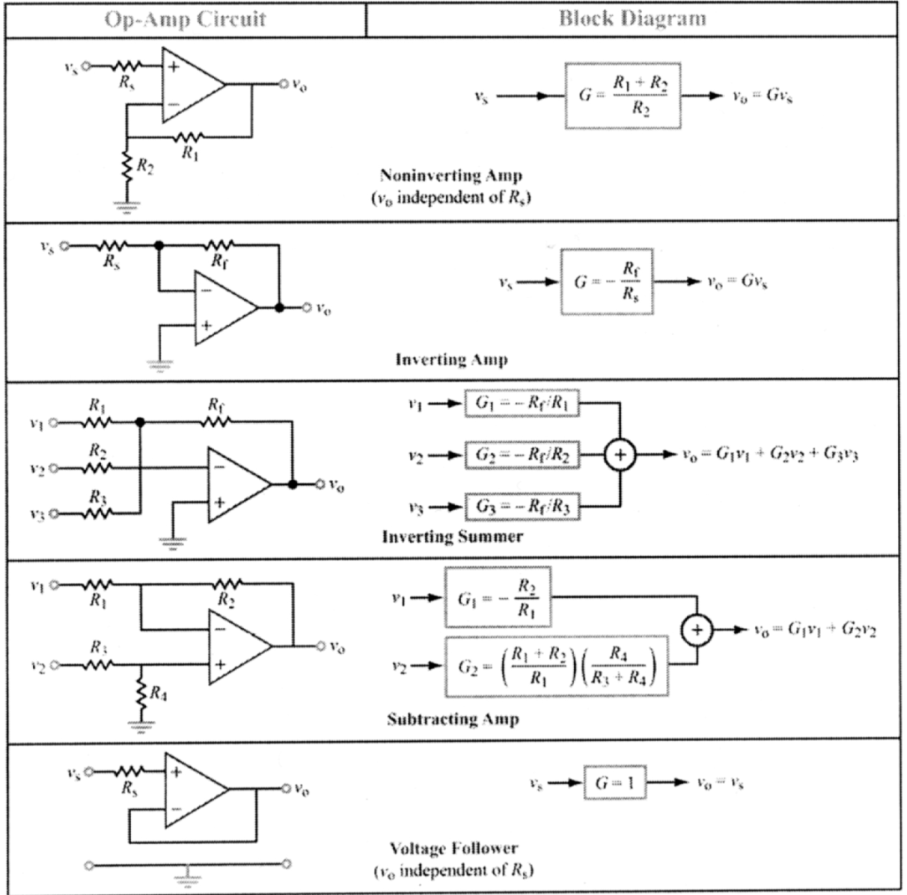
\includegraphics[width=.9\textwidth]{Figures/OPAMPS.png}
      \caption{OpAmp Shortcuts}
      \label{fig:1}
    \end{figure}
    
$$\boxed{i^1=i\,\,\,\,\,\,\,\,\,\,\,\,i^2=-1\,\,\,\,\,\,\,\,\,\,\,\,i^3=-i\,\,\,\,\,\,\,\,\,\,\,\,i^4=1}$$

\begin{multicols}{2}

Euler's Formula:

  $$\boxed{e^{j\theta}=\cos(\theta)+j\sin(\theta)}$$

  Amplitude: $\boxed{c=\sqrt{a^2+b^2}}$, where:

  $$\boxed{\left\{\begin{array}{c c} a &= c\cos(\theta)\\b &= c\sin(\theta)\end{array}}$$ 

Important properties:

  $$\boxed{a+jb=ce^{j\theta}}$$

  $$\boxed{\tan(\theta)=\frac{b}{a}}$$

Rectangular Form:

  $$\boxed{n=a+jb}$$

Polar Form:

  $$\boxed{n=ce^{j\theta}}$$

\end{multicols}

    \renewcommand{\arraystretch}{2.5}
  \begin{center}
    \begin{tabular}[H]{| l c c c |}
      \hline
      Property & $R$ & $L$ & $C$\\
      \hline
      $i-v$ relation & $i=\dfrac{v}{R}$ & $i=\dfrac{1}{L}\displaystyle \int_{t_0}^t v\,dt + i(t_0)$ & $i=C\dfrac{dv}{dt}$\\
      $v-i$ relation & $v=iR$ & $v=L\dfrac{di}{dt}$ & $v=\dfrac{1}{C}\displaystyle \int_{t_0}^t i\,dt+v(t_0)$\\
      $p$ (power transfer in) & $p=i^2R$ & $p=Li\dfrac{di}{dt}$ & $p=Cv\dfrac{dv}{dt}$\\
      $w$ (stored energy) & 0 & $w=\frac{1}{2}Li^2$ & $w=\frac{1}{2}Cv^2$\\
      Series Combination & $R_{eq}=R_1+R_2$ & $L_{eq}=L_1+L_2$ & $\dfrac{1}{C_{eq}}=\dfrac{1}{C_1}+\dfrac{1}{C_2}$\\
      Parallel Combination & $\dfrac{1}{R_{eq}}=\dfrac{1}{R_1}+\dfrac{1}{R_2}$ & $\dfrac{1}{L_{eq}}=\dfrac{1}{L_1}+\dfrac{1}{L_2}$ & $C_{eq}=C_1+C_2$\\
      DC Behavior & No change & Short circuit & Open circuit \\
      Instantaneous $v$ change? & Yes & Yes & No\\
      Instantaneous $i$ change? & Yes & No & Yes\\
      \hline
    \end{tabular}
  \end{center}

  \begin{multicols}{2}

    $$\boxed{i(t)=I_{\infty}+(I_o-I_{\infty})e^{-\dfrac{t}{\tau}}}$$

    $$\boxed{v(t)=V_{\infty}+(V_o-V_{\infty})e^{-\dfrac{t}{\tau}}}$$

  \end{multicols}

  \renewcommand{\arraystretch}{1.5}
  \begin{center}
    \begin{tabular}{| c c c |}
      \hline
      & $RC$ & $RL$ \\
      $\tau$ & $RC$ & $L/R$\\
      \hline
    \end{tabular}
  \end{center}

  $$\boxed{p = P + P\cos(2\omega t) - Q\sin(2\omega t)}$$

  \begin{center}
    Where:
  \end{center}

  \begin{multicols}{2}

    Average Power:

    $$\boxed{P=\dfrac{V_mI_m}{2}\cos(\theta_v - \theta_i}$$

    Reactive Power:

    $$\boxed{P=\dfrac{V_mI_m}{2}\sin(\theta_v - \theta_i}$$

  \end{multicols}

    Power Factor $$=\cos(90+\theta_v-\theta_i)$$

    \textsc{If} positive, power factor is leading

    \textsc{If} negative, power factor is lagging\\

    Maximum power transfer occurs when the Thevnin impedance is equal to the conjugate of the load impedance\\

    Fourier Series:

    $$\boxed{f(t)=a_0+\sum_{n=1}^{\infty} \left(a_n\cos(n\omega_0t)+b_n\sin(n\omega_0t)\right)}$$

    The coefficients of a Fourier series are:

 $$\mathcal{F}\left\{\begin{array}{c} a_0=\dfrac{1}{T}\displaystyle \int_0^T f(t)\,dt\\ a_k=\dfrac{2}{T}\displaystyle\int_0^T f(t)\cos(k\omega_0t)\,dt\\b_k=\dfrac{2}{T}\displaystyle\int_0^T f(t)\sin(k\omega_0t)\,dt \end{array}$$

For an even function $(f(t)=f(-t))$:

  $$\mathcal{F}\left\{\begin{array}{c} a_0=\dfrac{2}{T}\displaystyle \int_0^{\frac{T}{2}} f(t)\,dt\\ a_k=\dfrac{4}{T}\displaystyle\int_0^{\frac{T}{2}} f(t)\cos(k\omega_0t)\,dt\\b_k=0 \end{array}$$

For an odd function $(f(t)=-f(-t))$:

  $$\mathcal{F}\left\{\begin{array}{c} a_0=0\\ a_k=0\\ b_k=\dfrac{4}{T}\displaystyle\int_0^{\frac{T}{2}} f(t)\sin(k\omega_0t)\,dt\\ \end{array}$$

\begin{center}
    \begin{figure}[h!]
      \centering
      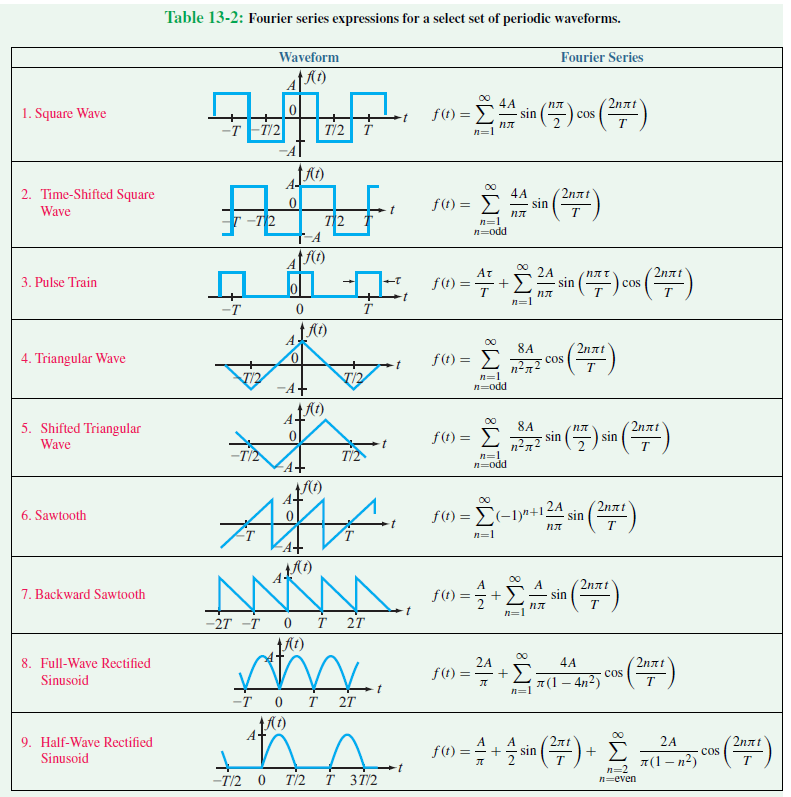
\includegraphics[width=.9\textwidth]{Figures/FT.png}
      \caption{Common Fourier Series Table}
      \label{fig:2}
    \end{figure}
  \end{center}

The Fourier transform is written as:

    $$F(\omega)=\mathcal{F}\{f(t)\}=\int_{-\infty}^{\infty}f(t)e^{-j\omega t}\,dt$$

    The transforms below are with respect to $-\infty \leq t\leq \infty$, other boundaries must be recalculated

    \begin{figure}[H]
      \centering
      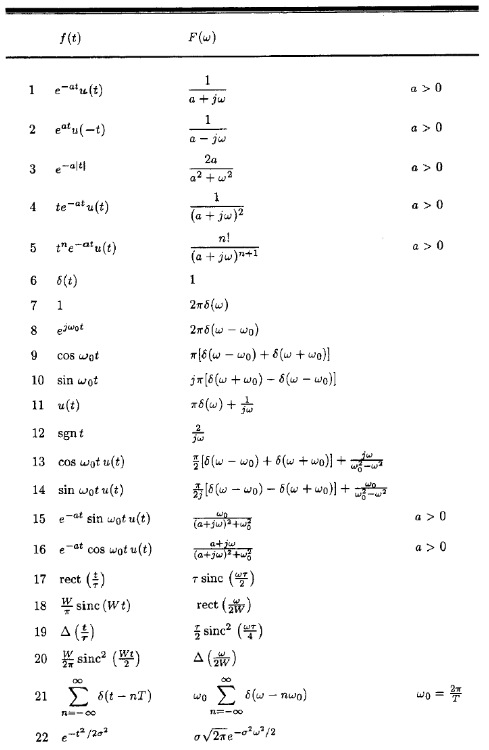
\includegraphics[height=.9\textheight]{Figures/FTT.png}
      \caption{Table of Common Fourier Transforms}
      \label{fig:3}
    \end{figure}

      \begin{figure}[H]
        \centering
        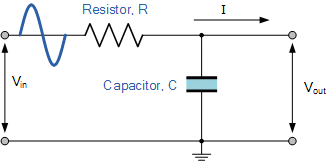
\includegraphics[width=.45\textwidth]{Figures/PLP.png}
        \caption{Passive Low Pass Filter $\left( f_c=\frac{1}{2\pi RC} \right)$}
        \label{fig:4}
      \end{figure}

      \begin{figure}[H]
        \centering
        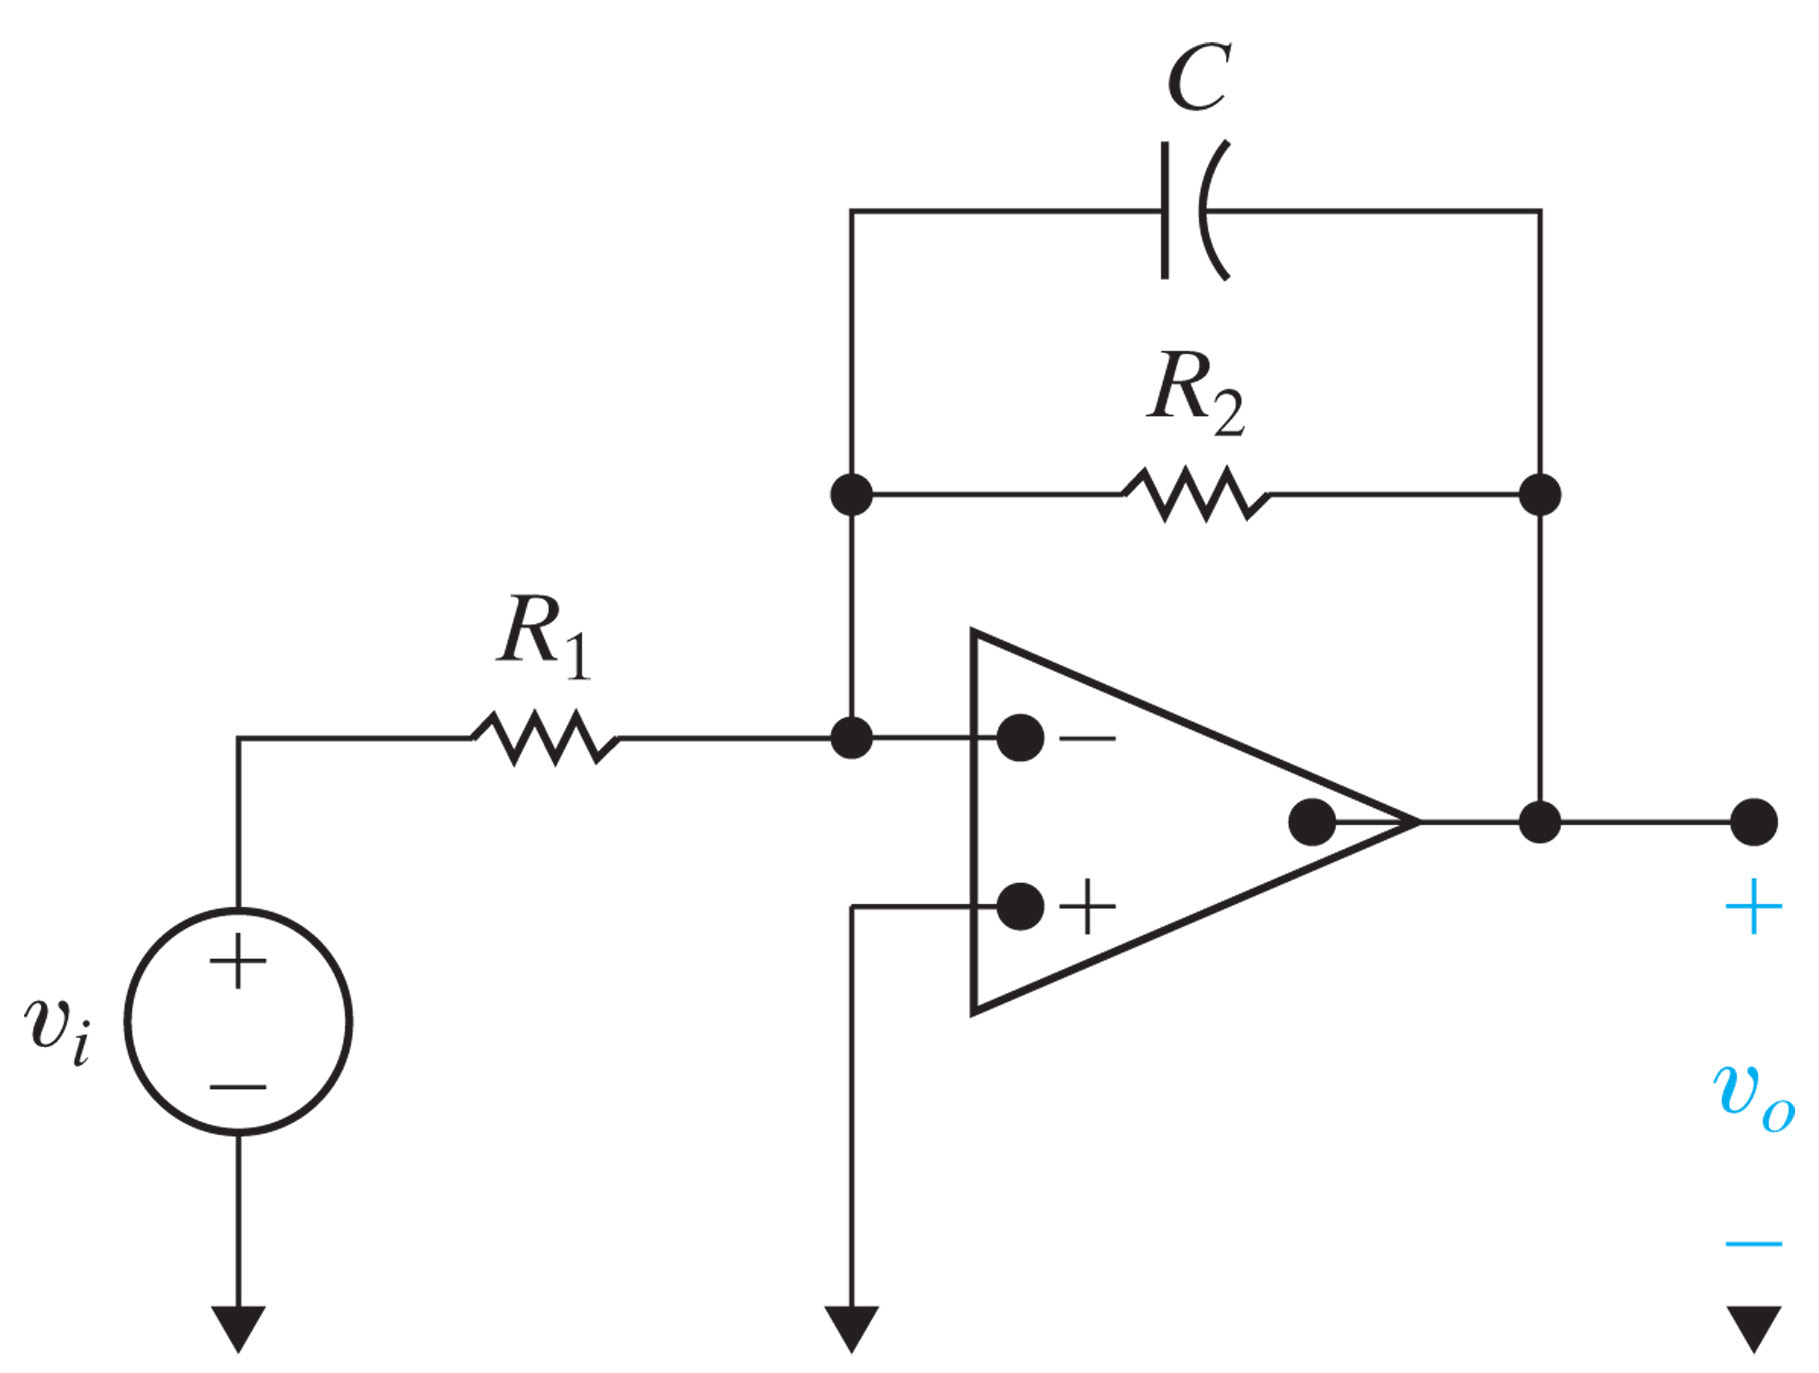
\includegraphics[width=.45\textwidth]{Figures/ALP.png}
        \caption{First Order Active Low Pass Filter}
        \label{fig:5}
      \end{figure}

      \begin{figure}[H]
        \centering
        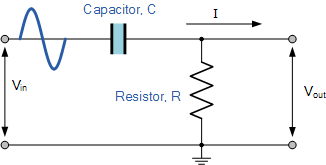
\includegraphics[width=.45\textwidth]{Figures/PHP.png}
        \caption{Passive High Pass Filter $\left( f_c=\frac{1}{2\pi RC} \right)$}
        \label{fig:6}
      \end{figure}

      \begin{figure}[H]
        \centering
        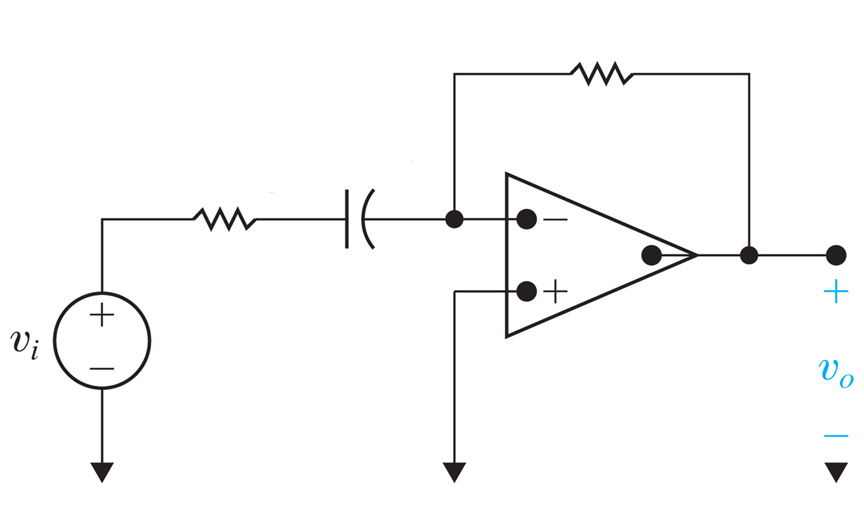
\includegraphics[width=.45\textwidth]{Figures/AHP.png}
        \caption{First Order Active High Pass Filter}
        \label{fig:7}
      \end{figure}

\end{document}

